\documentclass{standalone}
\usepackage{tikz}
\usetikzlibrary{patterns, positioning}

\begin{document}
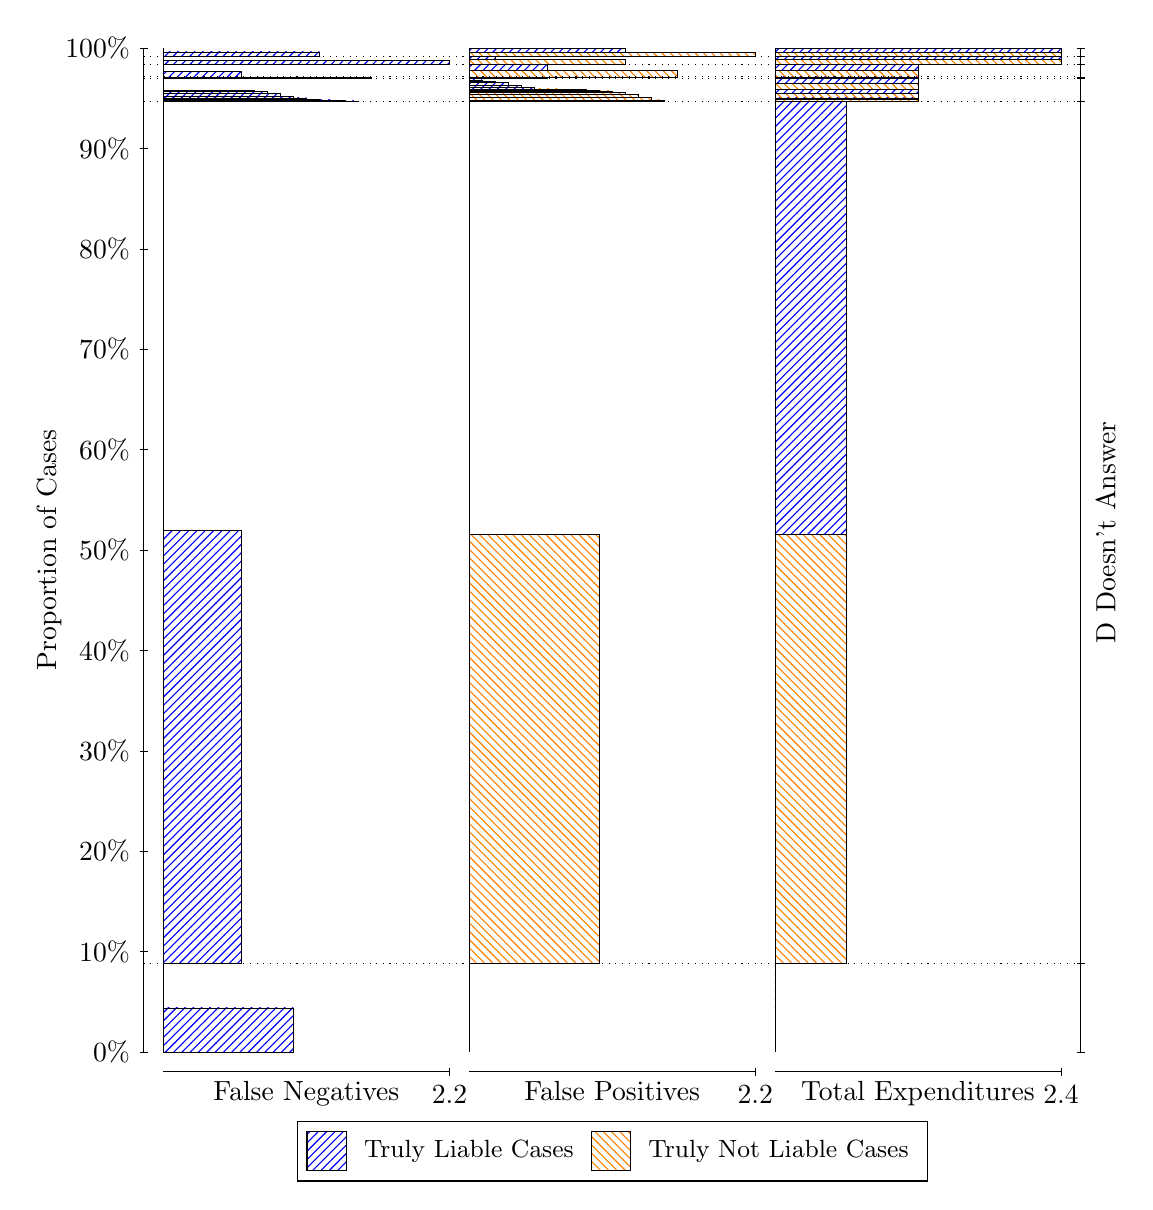
\begin{tikzpicture}
\draw[black, very thin] (1.5,1.75) -- (1.5,14.5);
\node[rotate=90, anchor=center] at (0.3, 8.125) {Proportion of Cases};
\draw[black, very thin] (1.45,1.75) -- (1.55,1.75);
\node[anchor=east] at (1.45, 1.75) {0\%};
\draw[black, very thin] (1.45,3.025) -- (1.55,3.025);
\node[anchor=east] at (1.45, 3.025) {10\%};
\draw[black, very thin] (1.45,4.3) -- (1.55,4.3);
\node[anchor=east] at (1.45, 4.3) {20\%};
\draw[black, very thin] (1.45,5.575) -- (1.55,5.575);
\node[anchor=east] at (1.45, 5.575) {30\%};
\draw[black, very thin] (1.45,6.85) -- (1.55,6.85);
\node[anchor=east] at (1.45, 6.85) {40\%};
\draw[black, very thin] (1.45,8.125) -- (1.55,8.125);
\node[anchor=east] at (1.45, 8.125) {50\%};
\draw[black, very thin] (1.45,9.4) -- (1.55,9.4);
\node[anchor=east] at (1.45, 9.4) {60\%};
\draw[black, very thin] (1.45,10.675) -- (1.55,10.675);
\node[anchor=east] at (1.45, 10.675) {70\%};
\draw[black, very thin] (1.45,11.95) -- (1.55,11.95);
\node[anchor=east] at (1.45, 11.95) {80\%};
\draw[black, very thin] (1.45,13.225) -- (1.55,13.225);
\node[anchor=east] at (1.45, 13.225) {90\%};
\draw[black, very thin] (1.45,14.5) -- (1.55,14.5);
\node[anchor=east] at (1.45, 14.5) {100\%};

\draw[black, very thin] (13.4,1.75) -- (13.4,14.5);
\draw[black, very thin] (13.35,1.75) -- (13.45,1.75);
\node[anchor=west] at (13.35, 1.75) {};
\draw[black, very thin] (13.35,2.8711) -- (13.45,2.8711);
\node[anchor=west] at (13.35, 2.8711) {};
\draw[black, very thin] (13.35,13.825) -- (13.45,13.825);
\node[anchor=west] at (13.35, 13.825) {};
\draw[black, very thin] (13.35,14.117) -- (13.45,14.117);
\node[anchor=west] at (13.35, 14.117) {};
\draw[black, very thin] (13.35,14.133) -- (13.45,14.133);
\node[anchor=west] at (13.35, 14.133) {};
\draw[black, very thin] (13.35,14.295) -- (13.45,14.295);
\node[anchor=west] at (13.35, 14.295) {};
\draw[black, very thin] (13.35,14.398) -- (13.45,14.398);
\node[anchor=west] at (13.35, 14.398) {};
\draw[black, very thin] (13.35,14.5) -- (13.45,14.5);
\node[anchor=west] at (13.35, 14.5) {};

\draw[black, very thin, pattern color=blue, pattern=north east lines] (1.75,1.75) rectangle (3.4015,2.3106);
\draw[black, very thin, pattern color=orange, pattern=north west lines] (1.75,2.3106) rectangle (1.75,2.8711);
\draw[black, very thin, pattern color=blue, pattern=north east lines] (1.75,2.8711) rectangle (2.7409,8.3702);
\draw[black, very thin, pattern color=orange, pattern=north west lines] (1.75,8.3702) rectangle (1.75,13.825);
\draw[black, very thin, pattern color=blue, pattern=north east lines] (1.75,13.825) rectangle (4.2273,13.828);
\draw[black, very thin, pattern color=blue, pattern=north east lines] (1.75,13.828) rectangle (4.0621,13.833);
\draw[black, very thin, pattern color=blue, pattern=north east lines] (1.75,13.833) rectangle (3.897,13.84);
\draw[black, very thin, pattern color=blue, pattern=north east lines] (1.75,13.84) rectangle (3.7318,13.847);
\draw[black, very thin, pattern color=blue, pattern=north east lines] (1.75,13.847) rectangle (3.5667,13.866);
\draw[black, very thin, pattern color=blue, pattern=north east lines] (1.75,13.866) rectangle (3.4015,13.882);
\draw[black, very thin, pattern color=blue, pattern=north east lines] (1.75,13.882) rectangle (3.2364,13.92);
\draw[black, very thin, pattern color=blue, pattern=north east lines] (1.75,13.92) rectangle (3.0712,13.946);
\draw[black, very thin, pattern color=blue, pattern=north east lines] (1.75,13.946) rectangle (2.9061,13.96);
\draw[black, very thin, pattern color=orange, pattern=north west lines] (1.75,13.96) rectangle (1.75,14.117);
\draw[black, very thin, pattern color=blue, pattern=north east lines] (1.75,14.117) rectangle (4.3924,14.125);
\draw[black, very thin, pattern color=orange, pattern=north west lines] (1.75,14.125) rectangle (1.75,14.133);
\draw[black, very thin, pattern color=blue, pattern=north east lines] (1.75,14.133) rectangle (2.7409,14.208);
\draw[black, very thin, pattern color=orange, pattern=north west lines] (1.75,14.208) rectangle (1.75,14.295);
\draw[black, very thin, pattern color=blue, pattern=north east lines] (1.75,14.295) rectangle (5.3833,14.339);
\draw[black, very thin, pattern color=orange, pattern=north west lines] (1.75,14.339) rectangle (1.75,14.398);
\draw[black, very thin, pattern color=blue, pattern=north east lines] (1.75,14.398) rectangle (3.7318,14.45);
\draw[black, very thin, pattern color=orange, pattern=north west lines] (1.75,14.45) rectangle (1.75,14.5);
\draw[black, very thin, pattern color=orange, pattern=north west lines] (5.6333,1.75) rectangle (5.6333,2.3106);
\draw[black, very thin, pattern color=blue, pattern=north east lines] (5.6333,2.3106) rectangle (5.6333,2.8711);
\draw[black, very thin, pattern color=orange, pattern=north west lines] (5.6333,2.8711) rectangle (7.2848,8.3256);
\draw[black, very thin, pattern color=blue, pattern=north east lines] (5.6333,8.3256) rectangle (5.6333,13.825);
\draw[black, very thin, pattern color=orange, pattern=north west lines] (5.6333,13.825) rectangle (8.1106,13.841);
\draw[black, very thin, pattern color=orange, pattern=north west lines] (5.6333,13.841) rectangle (7.9455,13.871);
\draw[black, very thin, pattern color=orange, pattern=north west lines] (5.6333,13.871) rectangle (7.7803,13.916);
\draw[black, very thin, pattern color=orange, pattern=north west lines] (5.6333,13.916) rectangle (7.6152,13.934);
\draw[black, very thin, pattern color=orange, pattern=north west lines] (5.6333,13.934) rectangle (7.45,13.956);
\draw[black, very thin, pattern color=orange, pattern=north west lines] (5.6333,13.956) rectangle (7.2848,13.963);
\draw[black, very thin, pattern color=orange, pattern=north west lines] (5.6333,13.963) rectangle (7.1197,13.972);
\draw[black, very thin, pattern color=orange, pattern=north west lines] (5.6333,13.972) rectangle (6.9545,13.977);
\draw[black, very thin, pattern color=orange, pattern=north west lines] (5.6333,13.977) rectangle (6.7894,13.981);
\draw[black, very thin, pattern color=blue, pattern=north east lines] (5.6333,13.981) rectangle (6.4591,13.996);
\draw[black, very thin, pattern color=blue, pattern=north east lines] (5.6333,13.996) rectangle (6.2939,14.021);
\draw[black, very thin, pattern color=blue, pattern=north east lines] (5.6333,14.021) rectangle (6.1288,14.059);
\draw[black, very thin, pattern color=blue, pattern=north east lines] (5.6333,14.059) rectangle (5.9636,14.075);
\draw[black, very thin, pattern color=blue, pattern=north east lines] (5.6333,14.075) rectangle (5.7985,14.095);
\draw[black, very thin, pattern color=blue, pattern=north east lines] (5.6333,14.095) rectangle (5.6333,14.117);
\draw[black, very thin, pattern color=orange, pattern=north west lines] (5.6333,14.117) rectangle (6.6242,14.125);
\draw[black, very thin, pattern color=blue, pattern=north east lines] (5.6333,14.125) rectangle (5.6333,14.133);
\draw[black, very thin, pattern color=orange, pattern=north west lines] (5.6333,14.133) rectangle (8.2758,14.22);
\draw[black, very thin, pattern color=blue, pattern=north east lines] (5.6333,14.22) rectangle (6.6242,14.295);
\draw[black, very thin, pattern color=orange, pattern=north west lines] (5.6333,14.295) rectangle (7.6152,14.354);
\draw[black, very thin, pattern color=blue, pattern=north east lines] (5.6333,14.354) rectangle (5.9636,14.398);
\draw[black, very thin, pattern color=orange, pattern=north west lines] (5.6333,14.398) rectangle (9.2667,14.449);
\draw[black, very thin, pattern color=blue, pattern=north east lines] (5.6333,14.449) rectangle (7.6152,14.5);
\draw[black, very thin, pattern color=orange, pattern=north west lines] (9.5167,1.75) rectangle (9.5167,2.3106);
\draw[black, very thin, pattern color=blue, pattern=north east lines] (9.5167,2.3106) rectangle (9.5167,2.8711);
\draw[black, very thin, pattern color=orange, pattern=north west lines] (9.5167,2.8711) rectangle (10.425,8.3256);
\draw[black, very thin, pattern color=blue, pattern=north east lines] (9.5167,8.3256) rectangle (10.425,13.825);
\draw[black, very thin, pattern color=orange, pattern=north west lines] (9.5167,13.825) rectangle (11.333,13.847);
\draw[black, very thin, pattern color=blue, pattern=north east lines] (9.5167,13.847) rectangle (11.333,13.866);
\draw[black, very thin, pattern color=orange, pattern=north west lines] (9.5167,13.866) rectangle (11.333,13.925);
\draw[black, very thin, pattern color=blue, pattern=north east lines] (9.5167,13.925) rectangle (11.333,13.978);
\draw[black, very thin, pattern color=orange, pattern=north west lines] (9.5167,13.978) rectangle (11.333,14.053);
\draw[black, very thin, pattern color=blue, pattern=north east lines] (9.5167,14.053) rectangle (11.333,14.117);
\draw[black, very thin, pattern color=orange, pattern=north west lines] (9.5167,14.117) rectangle (11.333,14.125);
\draw[black, very thin, pattern color=blue, pattern=north east lines] (9.5167,14.125) rectangle (11.333,14.133);
\draw[black, very thin, pattern color=orange, pattern=north west lines] (9.5167,14.133) rectangle (11.333,14.22);
\draw[black, very thin, pattern color=blue, pattern=north east lines] (9.5167,14.22) rectangle (11.333,14.295);
\draw[black, very thin, pattern color=orange, pattern=north west lines] (9.5167,14.295) rectangle (13.15,14.354);
\draw[black, very thin, pattern color=blue, pattern=north east lines] (9.5167,14.354) rectangle (13.15,14.398);
\draw[black, very thin, pattern color=orange, pattern=north west lines] (9.5167,14.398) rectangle (13.15,14.449);
\draw[black, very thin, pattern color=blue, pattern=north east lines] (9.5167,14.449) rectangle (13.15,14.5);
\draw[black, dotted] (1.5,2.8711) -- (13.4,2.8711);
\draw[black, dotted] (1.5,13.825) -- (13.4,13.825);
\draw[black, dotted] (1.5,14.117) -- (13.4,14.117);
\draw[black, dotted] (1.5,14.133) -- (13.4,14.133);
\draw[black, dotted] (1.5,14.295) -- (13.4,14.295);
\draw[black, dotted] (1.5,14.398) -- (13.4,14.398);
\draw[black, very thin] (1.75,1.5) -- (5.3833,1.5);
\node[anchor=north] at (3.5667, 1.5) {False Negatives};
\draw[black, very thin] (5.3833,1.45) -- (5.3833,1.55);
\node[anchor=north] at (5.3833, 1.45) {2.2};

\draw[black, very thin] (5.6333,1.5) -- (9.2667,1.5);
\node[anchor=north] at (7.45, 1.5) {False Positives};
\draw[black, very thin] (9.2667,1.45) -- (9.2667,1.55);
\node[anchor=north] at (9.2667, 1.45) {2.2};

\draw[black, very thin] (9.5167,1.5) -- (13.15,1.5);
\node[anchor=north] at (11.333, 1.5) {Total Expenditures};
\draw[black, very thin] (13.15,1.45) -- (13.15,1.55);
\node[anchor=north] at (13.15, 1.45) {2.4};


\node[black, centered, rotate=90] at (13.72, 8.3479) {D Doesn't Answer};






\draw (7.449999999999999,1.5) node[draw=none] (baseCoordinate) {};
\begin{scope}[align=center]
        \matrix[scale=0.5, draw=black, below=0.5cm of baseCoordinate, nodes={draw}, column sep=0.1cm]{
            \node[rectangle, draw, minimum width=0.5cm, minimum height=0.5cm, pattern=north east lines, pattern color=blue] {}; &
            \node[draw=none, font=\small] (B) {Truly Liable Cases}; &
            \node[rectangle, draw, minimum width=0.5cm, minimum height=0.5cm, pattern=north west lines, pattern color=orange] {}; &
            \node[draw=none, font=\small] (B) {Truly Not Liable Cases}; \\
            };
\end{scope}

\end{tikzpicture}
\end{document}